\section{Introduction}
\label{sec:intro}

Evolving graphs, i.e. graphs that change over time, can be used to
represent a wide range of phenomena, including the Web, social
networks, communication and transportation networks, interaction
networks, metabolism pathways, and many others.  Researchers study
graph evolution rate and mechanisms, impact of specific events on
further evolution, spatial and spatio-temporal patterns.  A natural
question arises of how to logically represent the graph evolution over
time such that the representation can support these operations.

\begin{figure}[b]
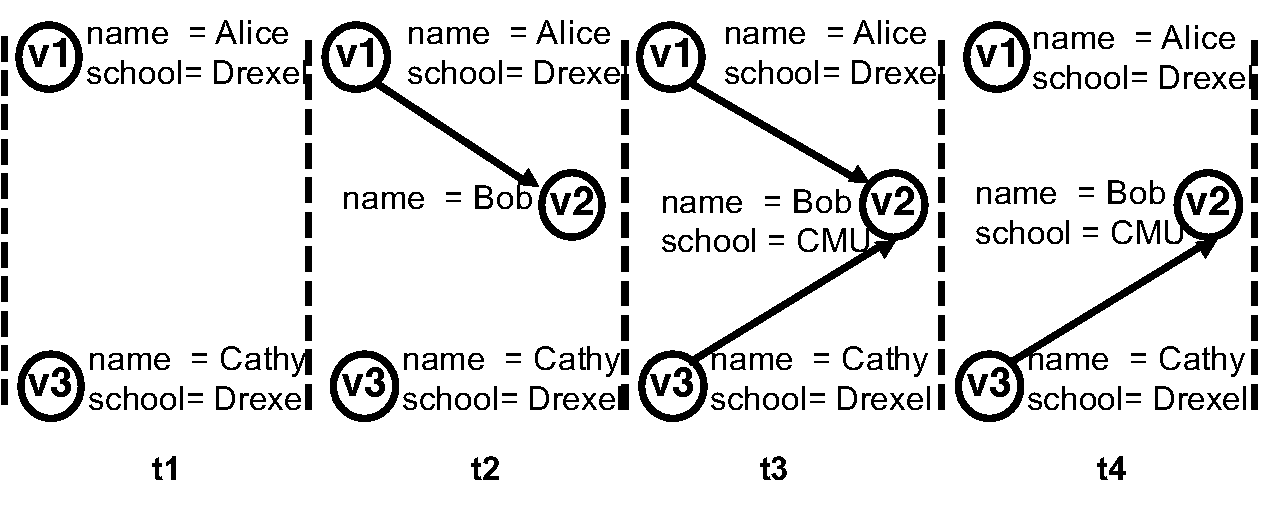
\includegraphics[width=3.4in]{figs/T1_graphs.pdf}
\vspace{-0.5cm}
\caption{Example social network as a snapshot sequence.}
%\vspace{-0.4cm}
\label{fig:snapshots}
\end{figure}

For historical reasons the dominant logical model for evolving graphs
in the research literature over the past 20 years has been a sequence
of static graphs, termed {\em snapshots}.  This model introduces a
semantic ambiguity that has been well studied in the temporal
relational databases literature~\cite{Bohlen1998}: if an entity,
i.e. node or edge, with the same attributes exists in two consecutive
snapshots, does it represent the same thing or a different one?  What
does it mean for an entity to change?  Figure~\ref{fig:snapshots}
shows an example evolving social network over four time points.  The
nodes in this network are people, while the edges are the interactions
between them such as likes and conversations.  In our example, did
Alice and Bob have two conversations over time period $[t1, t4)$ or
  one long one?  Did Alice undergo any changes during this time?  What
  is the rate of change of this evolving graph?  Which user was the
  most active in this network over its lifetime?  We cannot answer
  these questions without additional information based on this model.
  Perhaps Alice had a temporary position at Drexel at time $t1$ and
  was able to get a permanent one at time $t2$.  Alice and Bob had two
  interactions, while Cathy and Bob had one longer one.

This kind of semantic ambiguity affects several graph operations, most
notably aggregation and retrieval of change history, and, as a result,
global and local analytics that are useful in evolving graphs.

\begin{figure}[t]
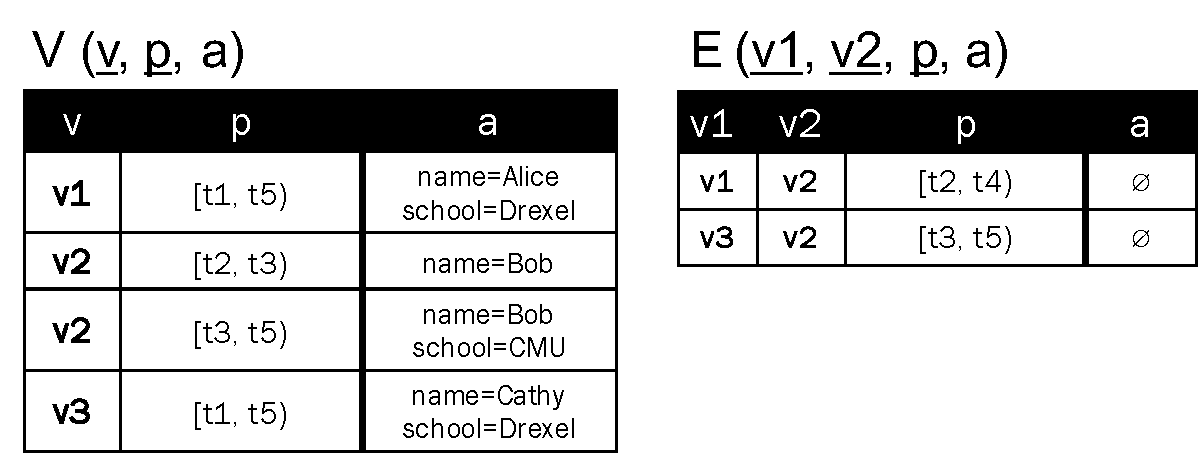
\includegraphics[width=3in]{figs/T1_relations.pdf}
%\vspace{-0.5cm}
\caption{Coalesced temporal relations representing evolving graph in Figure~\ref{fig:snapshots}.}
\vspace{-0.4cm}
\label{fig:coalesced}
\end{figure}

A snapshot sequence is a graph-specific adaptation of the point-based
time model~\cite{Toman2009}.  In point-based models each entity is
time-stamped with its validity time.  For practical considerations
intervals are often used as syntactic abbreviations for sets of
points, as the pure point-based model is obviously inefficient.
However, the use of intervals to represent a sequence of equivalent
time-adjacent snapshots is not semantically equivalent to an interval
model, where entities are time-stamped with intervals.  To use
intervals in a time-stamped model, we coalesce value-equivalent tuples
over overlapping and adjacent time points~\cite{Bohlen09}.  In
Figure~\ref{fig:coalesced} the result of coalesced representation from
Figure~\ref{fig:snapshots} is shown, using one temporal relation for
nodes and another for edges.  Attributes are represented as a set of
key-value pairs based on a property graph model~\cite{Angles2008}.
Note that Alice shows no changes during the whole time interval, with
a single tuple over $[t1, t4)$.  Similarly, two interactions between
  Alice and Bob are coalesced into one.  A work-around for this
  situation is to add additional attributes to entities in order to
  distinguish between changes and non-changes.  We can add position
  title to Alice node and conversation id to each edge.  This solution
  is ad-hoc rather than general and does not hold up over long periods
  of time when different changes appear.

We contend that a snapshot sequence point-based model of evolving
graphs is insufficient for representation of a wide range of networks.
This particularly affects interaction networks, such as message
exchange graphs, epidemic transmission networks, network topologies,
and any graphs with events as edges.  Instead we propose to use a
model with interval semantics instead.  In Section~\ref{sec:related}
we briefly survey existing models and summarize relevant work in
temporal databases.  We then propose a new model in
Section~\ref{sec:model} and discuss its properties.  In
Section~\ref{sec:consider} we address a few practical considerations
of model adoption and conclude with future research directions in
Section~\ref{sec:conc}.
